% vim: textwidth=78 ai spell spelllang=en
\documentclass[graybox]{svmult}

\usepackage[utf8x]{inputenc}
\usepackage[IL2]{fontenc}

\usepackage{mathptmx}       % selects Times Roman as basic font
\usepackage{helvet}         % selects Helvetica as sans-serif font
\usepackage{courier}        % selects Courier as typewriter font
\usepackage{type1cm}        % activate if the above 3 fonts are
                            % not available on your system
%
\usepackage{makeidx}         % allows index generation
\usepackage{graphicx}        % standard LaTeX graphics tool
                             % when including figure files
\usepackage[bottom]{footmisc}% places footnotes at page bottom

\makeindex             % used for the subject index
                       % please use the style svind.ist with
                       % your makeindex program

%%%%%%%%%%%%%%%%%%%%%%%%%%%%%%%%%%%%%%%%%%%%%%%%%%%%%%%%%%%%%%%%%%%%%%%%%%%%%%%%%%%%%%%%%

\begin{document}

\title*{Integrated Approach in Management and Design of Modern Web-Based
Services}
\author{Jaroslav Škrabálek and Lucia Tokarová and Jiří Slabý and Tomáš Pitner}
\institute{Jaroslav Škrabálek \at Faculty of Informatics, Masaryk
University, Brno, Czech Republic, \email{xskraba1@fi.muni.cz}
\and Lucia Tokarová \at Faculty of Informatics, Masaryk University,
Brno, Czech Republic, \email{xtokarov@fi.muni.cz}
\and Ji\v{r}í Slabý \at Faculty of Informatics, Masaryk University, Brno, Czech
Republic, \email{xslaby@fi.muni.cz}
\and Tomáš Pitner \at Faculty of Informatics, Masaryk University,
Brno, Czech Republic, \email{tomp@fi.muni.cz}}

\maketitle

\abstract*{TBD}

\abstract{TBD}

\section{Introduction}
Since the modern web-based services importance has arose among the software
development and ICT industry in general, significant changes in approach to
the software product can be seen. It does not matter whether we consider
classical desktop application or web application. But thanks to web
applications the process of changes has been catalysed and user is becoming
the primary factor determining the result form of product -- both from the
point of functionality and user interface.

Web technology advancements caused companies transition from desktop
applications to the Internet services. During this period, processes of the
web transformation have been replaced in favour of the higher level of
Internet development. The Internet from the Web 2.0 point of view is not only
a provider of static, passive information anymore.  The Internet became a
standalone platform offering \emph{Rich Internet Applications} (RIA) -- modern
web-based services \cite{o2007web}. Increasing complexity and usability of RIA
has changed people’s understanding not only of the Internet but the whole
process of developing such application, communication interface of that
application and the approach to people who creates the application in the end.
These significant questions regarding the software development
\cite{pitner-priklady}
are now broadly discussed and the process itself has been redefined. The most
important change is diverting from purely technological perception of final
software product to the consideration of product’s user acceptance. Not the
functionality is standing on the first place but usability. The change has
second major influence on developers where companies gradually turn their task
orientation to developer orientation where developers are carrier of the tasks
and potentially product success. The more developer will be satisfied the more
the task will be fulfilled in a satisfactory manner.

\section{Combining Disparate Technical and Humanistic Aspects in IT Project
Management}
Development of modern web-based services is very appropriate for application
in new humanistic management approaches with outlook emphasizing common human
needs since they are strongly oriented to the fundamental social principles of
their users. Social aspect for the modern web is essential. Whereas the
content of Web 2.0 is mainly user-generated, communities and collaboration are
highlighted. After very short period new Web 2.0 phenomena capture the heart
of millions Internet users. They are blogging, using wikies (which becomes
modern encyclopaedias), various community networks such a MySpace
(approximately 200 million users and slightly decreasing), Facebook (about 400
million users and growing), LinkedIn, XING, etc. One of the core concepts of
Web 2.0 became so called Folksonomy -- attaching unstructured -- a combination
of "folk" and "taxonomy". This concept was defined thanks to long interest of
Thomas Vander Wal (he observes phenomenon of tagging since the pre-web era in
1980s). Folksonomy represents process of tagging with social titling (social
indexing, social classification, collaborative tagging) of resources. Tagging
is very similar to the way how our brain works. It creates transcendent
manifold associations rather than inflexible categories. More plainly --
folksonomies are set of names tagged to the content by users without any fixed
predetermination. It is usually informal free form.

Human management in these days is characterised by acceptance of business
enterprise as an anthropomorphized being where persons in the enterprise
defines the culture and quality of the organization and their products as
well.  Organizations should build up unity to achieve that the community of
persons becomes stronger as a community \cite{mele2003challenge}. The business
cannot be
considered only as a ‘society of capital goods’ because it is also a ‘society
of persons’ \cite{paul1991centesimus}. Managers have to motivate people around
them to
acquire virtues and try to discover and promote beliefs and values within the
organizational culture that foster human virtue, in all its forms, to its
fullest extent. Humanity management is neither a naive approach nor a lack of
realism. It fulfils aim of the third approach to humanistic management, which
is still emerging, that considers a team as a real community of persons. The
connection to virtual community of Web 2.0 is obvious
\cite{motschnig2002learning}. This
humanistic project management approach is a real challenge in order to achieve
a higher moral quality in management and more efficient development and in the
end more efficient organizations, in fact. Only by this the full potential of
the organization -- mainly formed by the people -- will be exposed. Possible
aspects of person -- developer -- psychology development can be imagine as a
continuum encompassing training, conditioning, introjection and receptive
learning of foreign experiences. Personal values and project goal are in the
same level of importance and they get in the relationship between project
manager and developer. In that manner the growth process is created and sense
of personal and project development is higher.

Thanks to a close connection of Web 2.0 to the Person-Centered Approach via
Web 2.0 definition basis (e.g. collaborations, user-generated content, and
collective intelligence), it is an application of Web 2.0 technologies that
supplements original intention of Person-Centered Approach (PCA) properly
\cite{derntl2004r}. Person-Centered Approach was introduced by the American
psychologist Carl Rogers. The essentials are three attitudinal conditions
according to Rogers, which they are motive power in personal development of
each person. These conditions are:
\begin{itemize}
\item acceptance (unconditional positive regard),
\item emphatic understanding and
\item congruence.
\end{itemize}

Congruence expresses personal integrity composing from experiences and
feelings in mutual complementation. Integrity comprises acceptance and
emphatic understanding as well. Those attitudes are beneficial for all
relationships characterized by psychical development -- relationship between
child and parents, partners, or relationship between manager and developer
too. We called this Developer-Centered Approach (DCA). Through the changes
that Web 2.0 introduces to the software development the classical software
development and project management methodology adapts in methodology right for
the Internet environment. The PCA changes in certain point of view the
management methodology as well.

In order to choose proper Web 2.0 tools, special visual patterns and
specifications of PCA (or its specialization DCA) should be implemented during
the development of software products. But generally it does not matter whether
it is desktop application, web-based services or modern mobile application in
the end. The fundamental approach shall be the same.

\begin{figure}
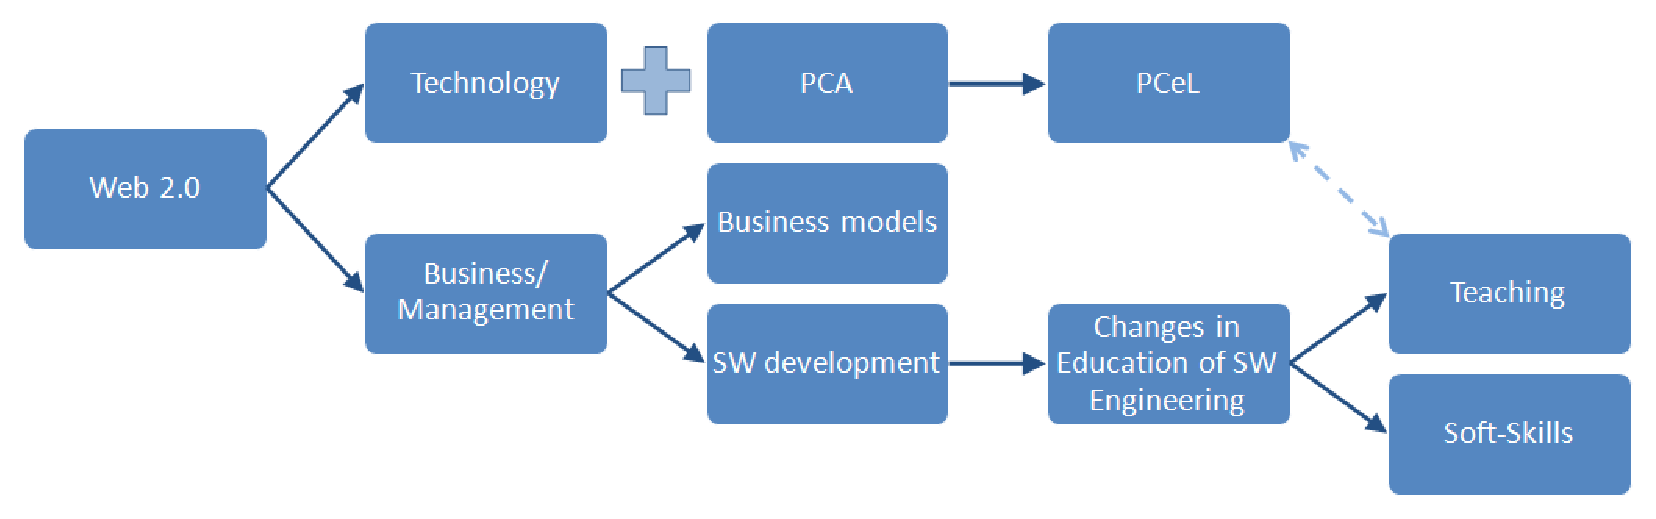
\includegraphics[width=\textwidth]{influence}
\caption{Influence of Web 2.0 in Technology Advancement, Project and Business
Management resulting in Education}
\end{figure}

The differences that Web 2.0 brings to ICT have important impact on project
management of these services \cite{vossen2007unleashing} from technical point
of view.
Special features of modern-web based services such a  development stage of
"perpetual beta", absence of software release cycle, dynamic scalability,
lightweight programming models, sampling and testing, etc. requires special
approaches being distinguished from the classical ones [O’Reilly, 07]. Many
books have been written about project management and surely many will appear
in the future. Basis of planning a software project, estimating its workload,
building a schedule, gathering software requirements and creating use cases,
improving programming with refactoring, unit testing, version control and
testing software are well known. So far we encountered with approaches and
software development processes which have been established and introduced into
the practise \cite{stellman2005applied} such a simple model the Waterfall,
Critical Chain Project Management, Extreme Project Management including Scrum
and Agile
Software Development to the sophisticated methodologies like PRINCE2 or
Rational Unified Process by IBM. But those approaches mainly result from an
earlier degree of software development appropriate to desktop programs. Web
2.0 projects have significant differences such as a rapid deployment or
sharing the web-based services with many users with the ability of
collaborative work accessing the data wherever the users are, while desktop
programs are primarily used by one user, on one computer (or small local
network) using local computer (local network) resources.

From practical experience, \emph{Agile Project Management} is the closest
approach to satisfy Web 2.0 needs so far. It is quite new approach and
therefore agile methodology reflects the current development of ICT industry
tightly. Agile project management stands on simple idea of incremental or
iterative (depends on what you prefer) proceedings. Thanks to these developers
are able to react on changes in time, or eventually stop the whole project,
redefine it, etc.  With agile development the Scrum method is connected very
closely. The basis of Scrum is so called Product Backlog or in other words
wish list of all things that the product shall contain. In this phase often
unrealistic requirements are included in Product Backlog. However, immediately
the work on \emph{Release Backlog} starts which represents the implementation
plan of particular functionalities. There can be the first variance between
Web 2.0 definition and Scrum. In Web 2.0 we often do not have very detailed
implementation plans.  Surely even in Internet environment there has to be
controlling. But in pure understanding of Web 2.0, new functionality is added
according to the need of user, not the plan. Iteration cycle with reference to
Agile methodology and Scrum is Sprint which is relatively short period of time
(usually 7-30 days) which satisfies Web 2.0 very short deploying cycle.
Although RIA can be deployed very quickly e.g. each hour -- Flickr, famous
photosharing site, has an iteration cycle sometime a half an hour.

Therefore there is a need for project management approach combining such
classical methodologies with more complex approaches reflecting the necessity
of proper business models closely connected to the development, efficiency and
performance of RIA, security issues, etc. This modern approach shall not only
focus on the development itself but according to contemporary trends of
humanistic approaches (described above) to the developers who stay behind
every single project and the project’s success depends on them.

\section{Designing usability}
Designing usability introduces several requests. First of all, usability must
be related to concrete project or product. According to international standard
ISO 9241 \cite{iso9241-11}, usability is defined as: "The extent to which a
product can be used by specified users to achieve specified goals with
effectiveness, efficiency and satisfaction in a specified context of use."
This means, there is no guaranteed method, which can be applied to reach
satisfying results. The selection of suitable method or combination of methods
depends strongly on the particular project. However, there are several
recommendations which can help to develop usable system:

\begin{quotation}
\emph{Future users’ involvement}: Future users should be involved in the
process of development from the very beginning. In the stage of requirement
analysis,
they should be in the center of interest rather than technologies.
Requirements should take into account human perspective, needs, wishes and
limitations. To understand these aspects, it is important to engage users into
the process. In case of designing system that should support people while
performing certain kind of activities, it is appropriate to examine the
activities, ask people to explain what they like and do not like about the
current way of performing activities, observe them while working, look for
problems they have, and so on. Future users should also participate in later
development stages -- especially in system evaluation and usability testing.

The situation is more complicated, when future users are not known explicitly.
This is often the case of designing web applications -- development process is
not initiated by the needs of future users, it is rather started by the idea
of product owner and his business plan. In this situation, it is quite
difficult to predict future users’ requirements. Therefore it is suitable to
ask marketing department to develop profile of target audience for the
product. Characteristics of future users can be built upon the market research
and design process should be oriented on representative sample of future
customers.

\vspace{3mm}
\emph{Usability experts’ involvement}: Usability experts should be involved in
the process from the very beginning. To achieve best possible results,
usability
specialist or group of specialists should be devoted to deal with usability
issues as a part of the project development team. They can help with
specifying requirements, because they are experienced in using various
techniques to identify and understand users´ needs. They can suggest suitable
design approach -- select effective methods and techniques of usability
engineering for particular product. They can also identify usability errors
and find the solutions to fix them. However, their work should not be focused
primarily on error detection and elimination. The main reason of their
participation in the project should be matching design with users needs (Lund,
1997).

\vspace{3mm}
\emph{Iterative process}: Development process should be iterative. Process of
specifying requirements should evolve during the time -- initial requirements
are usually brief, they must be refined gradually and adjusted according to
situation. Iterations should be frequently discussed with future users,
evaluated and redesigned. In order to make this process easier and faster,
prototyping can be used. The main reason is to identify and eliminate errors
in requirement analysis, specification and design as soon as possible.
Removing error which is detected after implementation is much more expensive
and time-consuming in comparison with early detected error.
\end{quotation}

\section{Usability Engineering Techniques}
There is a wide range of techniques that can be used to develop usable and
user-centered system. Suitable combination for particular project can be, for
instance, selected from following activities:
\begin{itemize}
\item \emph{Requirement analysis:} user and task analysis, interview, group
interview, focus group, vision seminar process, survey, questionnaires,
observation, study of end-users' work and context of their work, \ldots
\item \emph{Prototyping:} low-fidelity, medium-fidelity, high-fidelity
prototypes; simulations of activities, evaluation and redesign of prototype
\item \emph{Usability testing:} user testing, thinking aloud, cognitive
walkthrough, heuristic evaluation, inspection.
\end{itemize}

\subsection{Integrating usability activities into development process}
Although user-centered approach leads to many benefits (not only on the side
of end-users; product owners and developers profit as well), it is usually
quite difficult to enforce it in practice.

First of all, usability is often seen as something additional. Designing
usability requires time and money. Discussion between users and developers is
mediated by usability experts. It means, that communication is more
time-consuming and involves more people. On the other hand, it is usually
easier and more effective for usability practitioners to transform users’
expectation into requirements, because they take human perspective into
account rather than technical requirements and limitations.

Other problem is, that functionality is usually preferred to usability.
Benefits of usability are not tangible.  Therefore, when it comes to decision,
whether to invest money and time in usability or in development of new
functions, functions are often prioritized. The problem is that specified
functions might not meet users’ needs. They are present in the final product
but since the end-users do not need them or do not know how to use them, they
are worthless. In general, it is useful trying to identify and focus on small
number of functions which are interesting for most users.

Even if requirements are specified properly, there are many ways how to supply
them. Developers often choose the way, which is technically easy to implement.
This might lead to formal accuracy but it does not satisfy users. Very common
situation is that developers claim that better solution would take too much
time to implement. Since they are responsible for technical part and other
people involved in the process often do not have competence and knowledge to
argue with this claim, it is usually taken for granted. Therefore in this
case, project manager reduce usability requirements in order to meet deadline
and budget.

Usability testing and system evaluation is also quite expensive and
time-consuming. Some companies might see this investment as additional,
because users will test the product in use. This is not only inappropriate
(because end-users have to cope with errors which leads to stress,
inefficiency and anger) it also sheds a bad light on the reputation of product
developers.

Other common problem with usability testing is that usability consultants are
involved only into this late stage of development process. They are invited to
perform user testing and evaluate final product. This is not convenient,
because errors detected in this stage are very difficult to fix. These errors
would be much easier and less expensive to eliminate in the early stages of
development.

Developing web applications introduces some additional challenges. The
life-cycle of web application is different form traditional software. First of
all, process of development usually does not have clearly defined
boundaries. It is rather on-going activity of fixing errors and adding new
features. Under these conditions it is difficult to determine individual
stages of development process and plan usability activities suitable for
particular stages.

In a sense, this might be an advantage. Iterative development process support
opportunity to find and fix usability errors and gradually improve
application. Moreover, it also provides opportunity to try innovative
solutions for usability problems.

On the other hand, this approach can be dangerous. Usability activities are
usually not part of the process. Usability is often evaluated afterwards --
only after new features are implemented. It means software is not
intentionally designed to be usable; it is rather created and later adjusted
to be acceptable.

Potential threats of this approach are general usability reports -- expert
evaluations of applications provided by usability practitioners according to a
set of general usability heuristics. These reports identify basic problems
without taking context of the project into account. Therefore the evaluation
is not always adequate and may lead to misinterpretation.

\section{Cost-Benefit Analysis of Usability}
The main reason why it is difficult to enforce usability in development
process is that benefits of usable product are quite abstract. Moreover, these
benefits are relative -- various groups of people are involved in the process
and each group has different perspective on evaluation of benefits and
different priorities. Therefore it is difficult to measure and evaluate
advantages and it is mostly impossible to transform all these advantages into
financial gain, which is often most significant decisive factor for project
managers. Main obstacle is the lack of metrics. Other problem is the need of
appropriate model which allows decision-makers to evaluate investment
systematically.

During the last decades, several models for justifying usability have emerged.
These models use cost-benefit analysis -- evaluation method for analyzing
projects for investment purposes. In general, this method contains three
stages: \textit{identifying the value of expected cost and benefits, analyzing
the relationship between these two values and making the investment decision}.
(Burril and Ellsworth, 1980)

In terms of cost-benefits analysis of usability, potential cost might be
expressed as amount of money spent on usability activities (salaries of
employees and consultants, training costs) and benefits might be counted in
connection with increased efficiency and productivity. The difference between
these two values is used to demonstrate the profit which usability engineering
brings to a project. (Lund, 1997)

XXX

XXX

XXX

Cost-benefit analysis might provide evidence for justifying usability
activities in development process. It tries to quantify possible benefits in
terms of return-on-investment, which is often significant decisive factor for
project managers.

However, there are still some problems left. Cost-benefit analysis is not
always compelling. It is rather retrospective approach. It can be used to
count gains of finished project, but it is more difficult to quantify profits
of oncoming project. In that case estimates are necessary. This might be a
source of inaccuracies. There are many variables, which are estimated, these
variables are multiplied and this leads to a significant bias. Moreover, these
variables are interdependent and there are too many side effects, which should
be taken into account (for example, when we want to estimate increase in
productivity of user of the new system, we have to measure the time for
performing activity; the problem is that time for performing activity differs
under normal circumstances and under stress circumstances and stress might be
a result of being tested).

More accurate estimations can be gained by more precise research. It means
more people involved, more time spent and as a result -- higher price. Other
source of data might be case studies of completed projects. This is also
problem -- product owners usually do not accept data of other companies as a
relevant source of information. Moreover, in practice there is a lack of this
kind of materials -- only few companies have published complete empirical case
study with original data.

Other problem of cost-benefit analysis is that various parties have different
perspectives. Different people consider different aspects as benefits.
Cost-benefit analysis can hardly cover and evaluate all possible gains. One
problem is diversity of benefits, other problem is the lack of metrics and
models to quantify them. Most profits are rather abstract and difficult to
express in terms of return-on-investment (for example reputation of company,
satisfaction of employees).

All these problems cause that cost-benefit analysis is not very common tool in
practice. Evaluation of cost and benefits of usability activities is usually
not conducted on its own, it is rather incorporated in cost-benefit analysis
of whole incoming project. However, in that time, it is too early to estimate
which activities might be necessary and what benefits might be gained.

In practice, it is usually conducted by usability consultants on customers
demand. It is not very often used as a tool which should enforce project
managers to invest money in usability activities.

Main reasons are time and financial demands, the lack of data about finished
projects and high possibility of inaccuracies.

On the other hand, cost-benefit analysis is the tool which is worth-knowing.
It can provide project managers with useful information, because models can be
used to evaluate costs and benefits of usability activities incorporated into
previous projects. Based on this evaluation, it is easier to predict what
activity is suitable for particular situation and what activity should be
avoided.

\section{Conclusions}

\section*{Acknowledgements}
The contribution is a part of the Project (No. 2615/2010/G1) called "New
Approaches to the Software Development Education" supported by the Ministry of
Education, Youth and Sports, Czech Republic.

\bibliographystyle{spbasic}
\bibliography{isd2010}
\end{document}
